% !TEX TS-program = xelatex
% !TEX encoding = UTF-8
% !Mode:: "TeX:UTF-8"

\documentclass[onecolumn,oneside]{SUSTechHomework}

\usepackage{float}
\usepackage{listings}
\lstset{
  language=Matlab,  %代码语言使用的是matlab
  frame=shadowbox, %把代码用带有阴影的框圈起来
%  rulesepcolor=\color{red!20!green!20!blue!20},%代码块边框为淡青色
%  keywordstyle=\color{blue!90}\bfseries, %代码关键字的颜色为蓝色,粗体
%  commentstyle=\color{red!10!green!70}\textit,    % 设置代码注释的颜色
  showstringspaces=false,%不显示代码字符串中间的空格标记
  numbers=left, % 显示行号
  numberstyle=\tiny,    % 行号字体
  stringstyle=\ttfamily, % 代码字符串的特殊格式
  breaklines=true, %对过长的代码自动换行
  extendedchars=false,  %解决代码跨页时,章节标题,页眉等汉字不显示的问题
%  escapebegin=\begin{CJK*},escapeend=\end{CJK*},      % 代码中出现中文必须加上,否则报错
  texcl=true
}

\author{胡玉斌}
\sid{11712121}
\title{Lab 7}
\coursecode{CS315}
\coursename{Computer Security}

\begin{document}
  \maketitle

  \section{Read the lab instructions above and finish all the tasks.}

  Done

  \section{Answer the questions and justify your answers.Simple yes or no answer will not get any credits.}

    \subsection{What is a zero-day attack?}

    \begin{itemize}
      \item A zero-day (also known as 0-day) vulnerability is a computer-software vulnerability that is unknown to those who should be interested in mitigating the vulnerability (including the vendor of the target software).
      \item Until the vulnerability is mitigated, hackers can exploit it to adversely affect computer programs, data, additional computers or a network.
      \item The term "zero-day" originally referred to the number of days since a new piece of software was released to the public, so "zero-day" software was software that had been obtained by hacking into a developer's computer before release. Eventually the term was applied to the vulnerabilities that allowed this hacking, and to the number of days that the vendor has had to fix them. Once the vendor learns of the vulnerability, the vendor will usually create patches or advise workarounds to mitigate it.
    \end{itemize}

    \subsection{Can Snort catch zero-day network attacks? If not, why not? If yes, how?}

      \begin{itemize}
        \item No
        \item Snort is one of the most popular open-source and rule-based IDSs.
        \item Its rules recognise malicious network packets by matching the current packet against predefined rules and cannot detect zero-day attacks but produce a high FPR due to its methodology for identifying attack signatures.
      \end{itemize}

    \subsection{Given a network that has 1 million connections daily where 0.1\% (not 10\%) are attacks. If the IDS has a true positive rate of 95\%, and the probability that an alarm is an attack is 95\%. What is false alarm rate? (You may use the math approach from the slides.)}

      \begin{itemize}
        \item[] $$\frac{ \mbox{TP}}{\mbox{TP}+\mbox{FP}}=95\%$$
        \item[] when $\mbox{TP}=950$, $\mbox{FP}=999000*r$, so we have:
        \item[] $$\frac{ \mbox{TP}}{\mbox{TP}+\mbox{FP}}=95\%$$
        \item[] So false alarm rate is $𝑟 = 0.005005\%$.
      \end{itemize}

  \section{Write a rule that will fire when you browse to craigslist.org or another particular website from the machine Snort is running on; it should look for any outbound TCP request to craigslist.org and alert on it.}

    \subsection{The rule you added(from the rules file)}

      \begin{itemize}
        \item We browse to sustech.edu.cn
        \item[] \begin{lstlisting}
alert tcp any any -> any any (msg:"SUSTech Packet found - Eveneko"; content:"sustech.edu.cn"; sid:1000002; rev:1;)
                \end{lstlisting}
      \end{itemize}

      \begin{figure}[H]
        \centering
        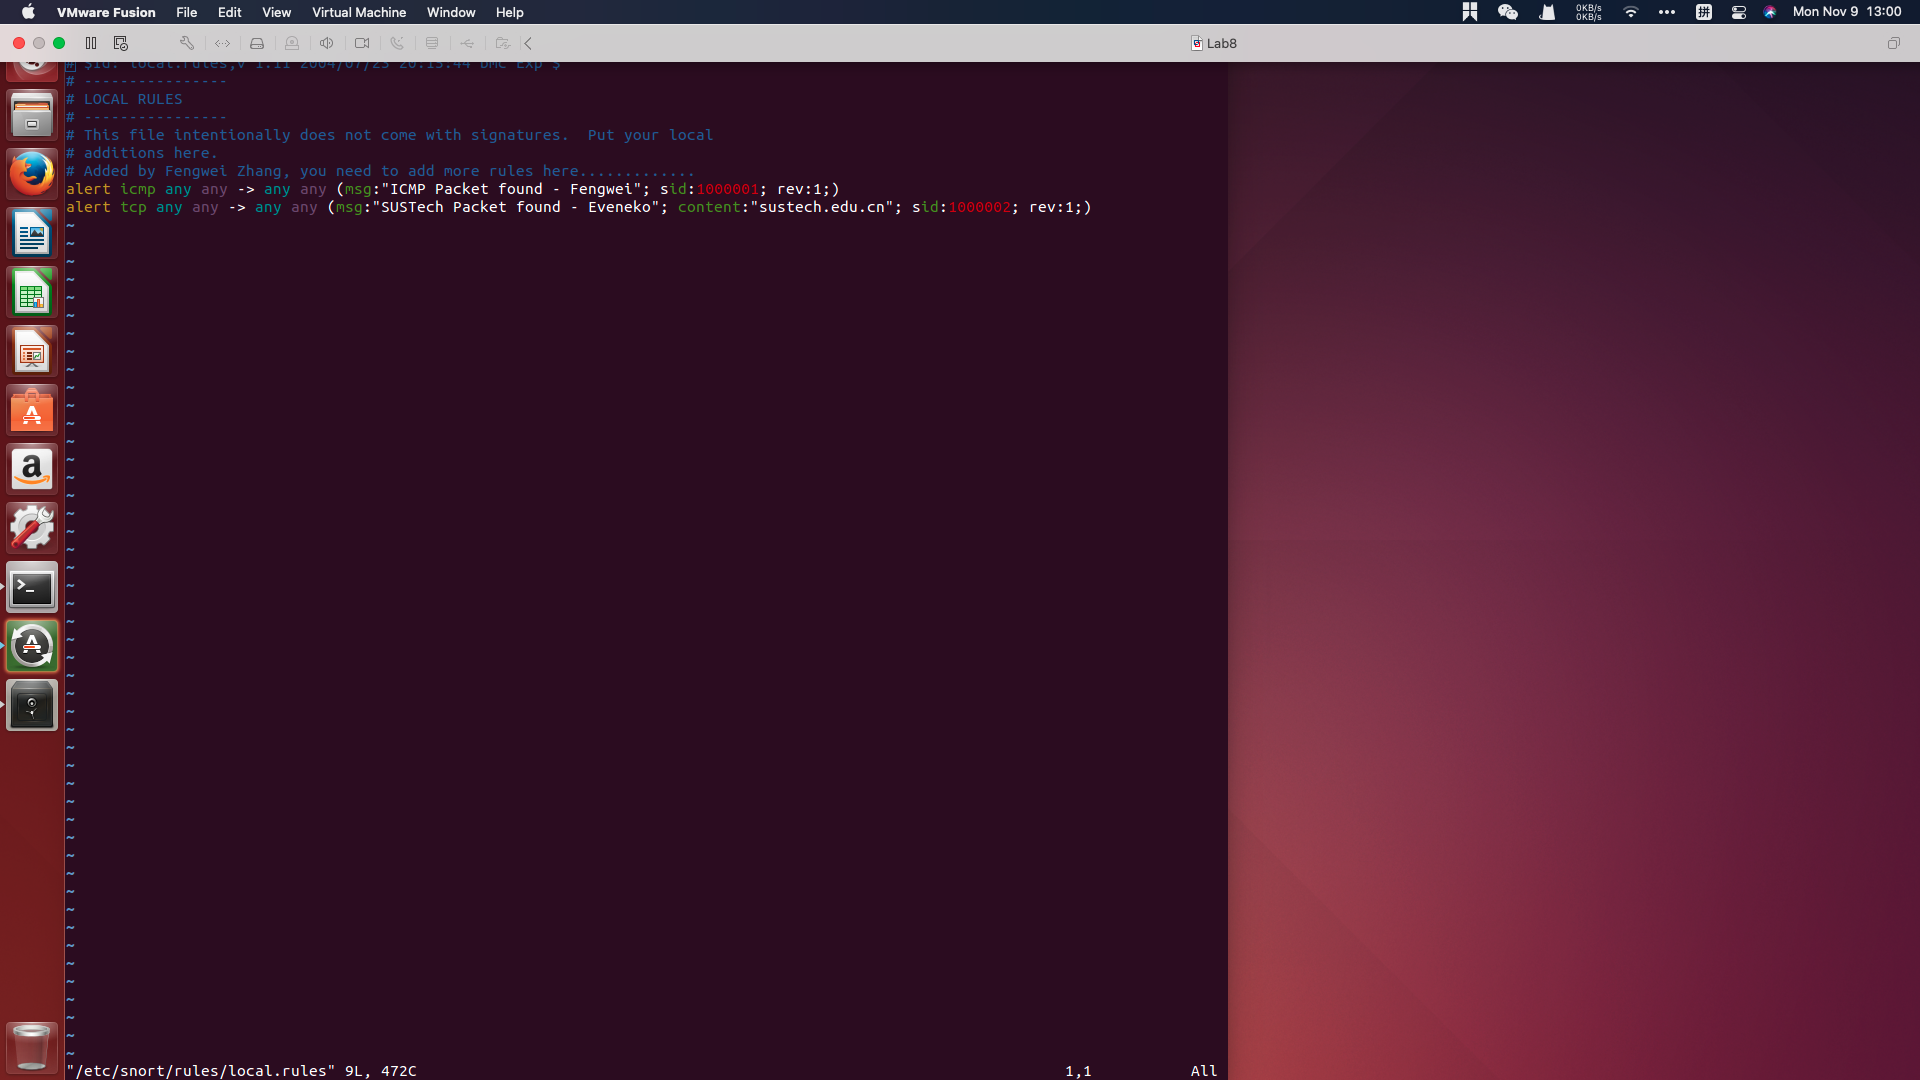
\includegraphics[width=0.85\textwidth]{img/pic1.png}
        \caption{rule}
      \end{figure}
  
    \subsection{A description of how you triggered the alert}

      \begin{figure}[H]
        \centering
        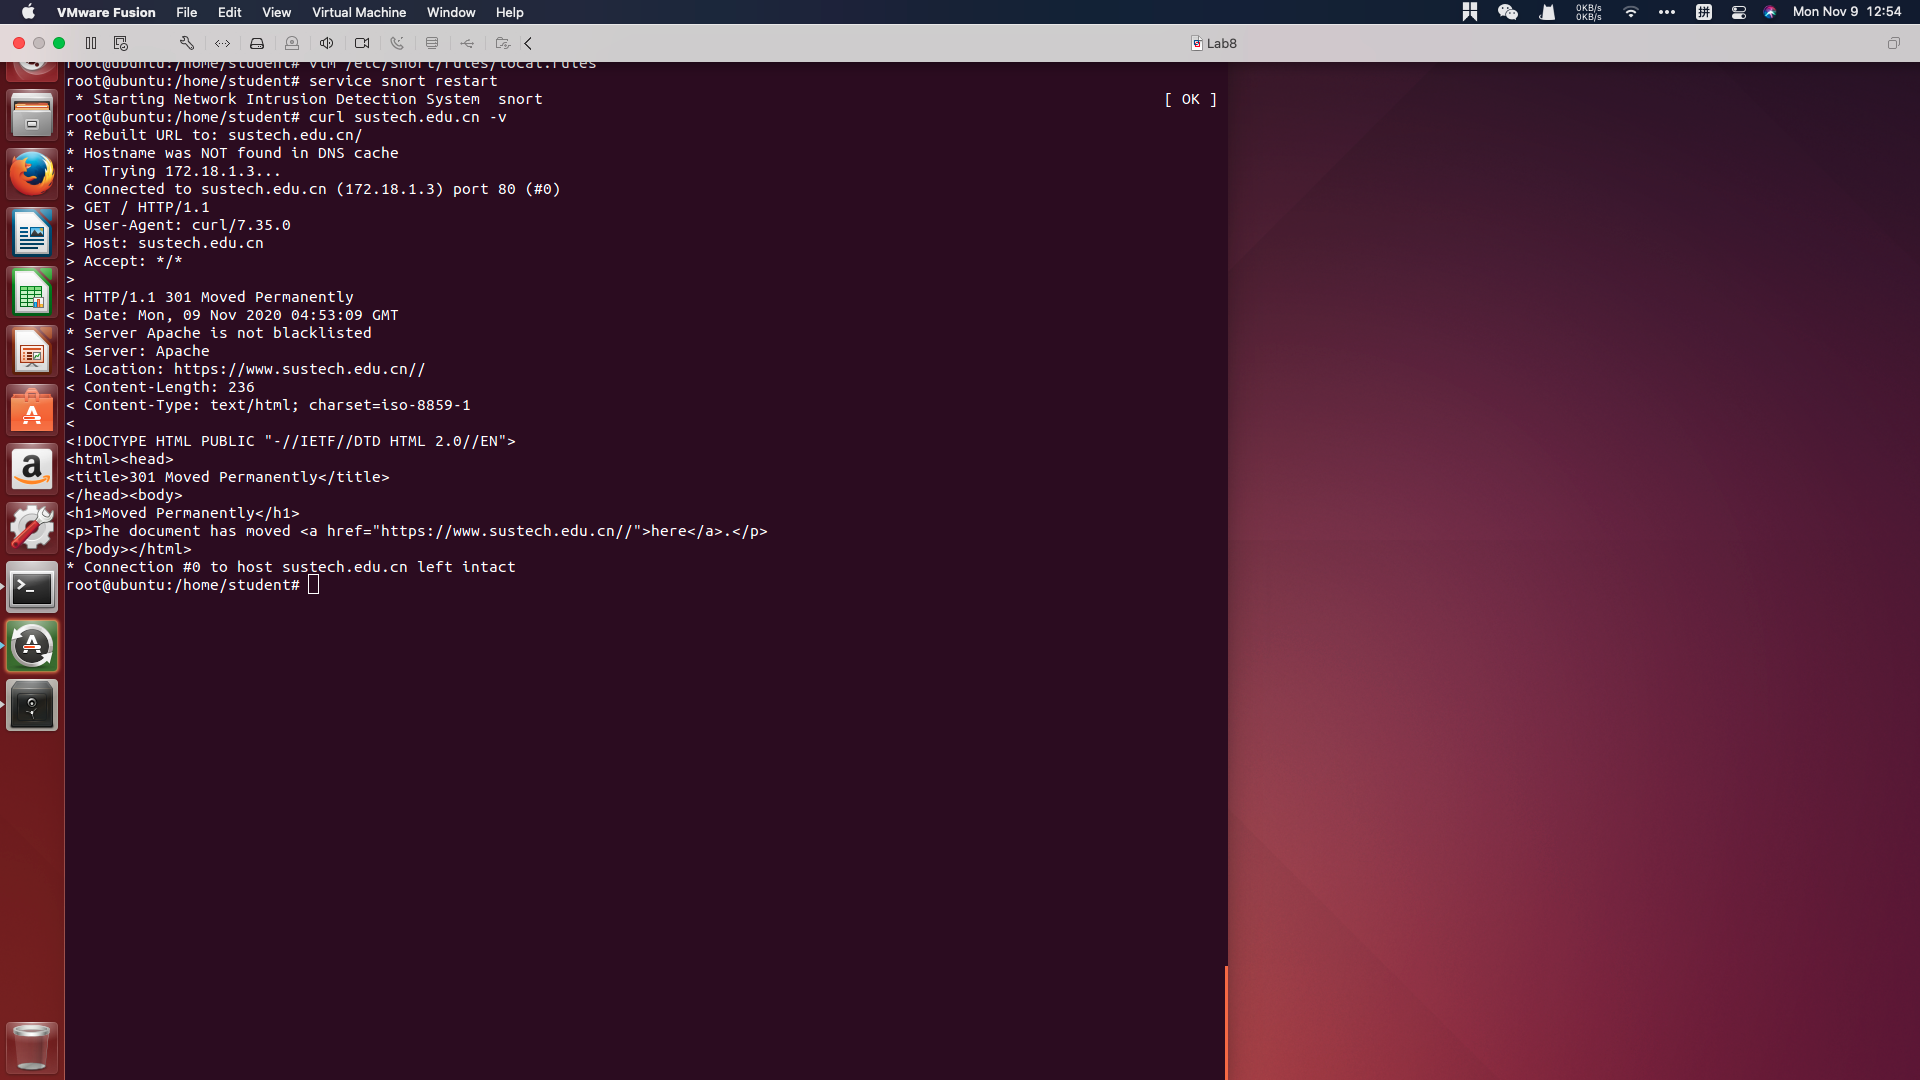
\includegraphics[width=0.85\textwidth]{img/pic2.png}
        \caption{trigger}
      \end{figure}

    \subsection{The alert itself from the log file (after converting it to readable text)}

      \begin{figure}[H]
        \centering
        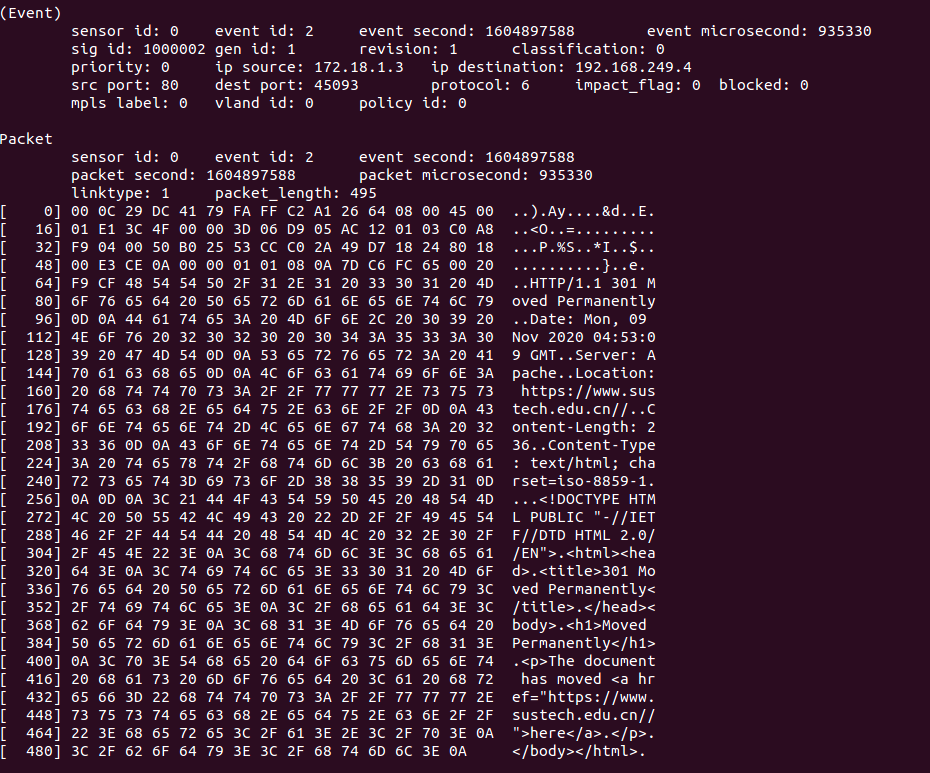
\includegraphics[width=0.85\textwidth]{img/pic3.png}
        \caption{log}
      \end{figure}
  
\end{document}
